\documentclass{report}

\usepackage[utf8]{inputenc}
\usepackage[italian]{babel}

\usepackage{mathtools}
\usepackage[tc]{titlepic}
\usepackage{graphicx}
\usepackage[margin = 1in]{geometry}

\usepackage{tikz}
\usepackage{pgfplots}
\pgfplotsset{
	width = .85\textwidth,
	height = .35\textheight
}



\DeclareUnicodeCharacter{00B0}{$ ^o$}
%workaround to dispay degree symbol


\title{
  \includegraphics[width = .7\textwidth]{titolo.png} \\[1cm]
  Laboratorio di Ottica, Elettronica e Fisica Moderna \\
  Interferometro di Michaelson \\
}
%\subtitle{Interferometro a Reticolo}
\author{
  Annoni Emilio, Delfrate Eleonora, Infurna Roberto \\
  Gruppo Me3 \\
}

\date{
  A.A. 2019/20 \\
  \today
  }

%%%%%%%%%%%%%%%%%%

\begin{document}


\section{Il Problema dell'osservatore lorenziano}


Le trasformazioni di Lorentz forniscono uno strumento per trasporre le informazioni che abbiamo in un sistema
di riferimento inerziale in un altro in moto rispetto a lui.
Porsi la domanda “che cosa vede ora l’altro osservatore”, per quanto relativa possa essere la risposta nel
mondo della Relatività, puo’ inoltre avere due interpretazioni.

\begin{itemize}
\item{
La prima riguarda l’idea fisica di “presente”, ovvero la configurazione del sistema ad un tempo t=0 per un
osservatore.
}
\item{
La seconda considera il processo fisico di “vedere” : io vedo ciò che in un passato più o meno remoto si è
trovato nel cammino della luce che arriva a me in questo momento.
}
\end{itemize}

Un’altra fonte di confusione nell’impostazione del problema sono le informazioni di cui siamo in possesso e che
usiamo per i calcoli: noi affermiamo di sapere tutto( con le dovute considerazioni come sarà chiaro più avanti)
del passato-presente-futuro di un sistema di riferimento privilegiato e fermo rispetto ad un nostro osservatore e
nel quale si muove un secondo osservatore per il quale vogliamo calcolare cosa vede.

La soluzione generale per entrambe i problemi seguirà lo stesso approccio e consisterà nel trovare l’istante di
tempo t nella storia dell’oggetto da visualizzare da utilizzare nella trasformazione, calcolato come presente per
l’altro osservatore.
La trasformazione di oggetti che sono fermi nel sistema preferenziale, a meno di un eventuale riscalamento non
richiederà calcoli.
Esiste in tutti e due una soluzione esatta se l’oggetto da visualizzare si muove di moto rettilineo uniforme,
mentre per un moto generico ciò non è a priori possibile.
E’ semplice dimostrare che se un oggetto si muove con velocità minore di quella della luce in qualsiasi sistema
di riferimento è o è stato “presente” o “visto” una e una sola volta.
Tenendo in memoria una porzione prefissata della storia di movimento del corpo, campionandone il movimento
ad intervalli discreti, sarà possibile attraverso bisezione identificare l’intervallo in cui l’oggetto attraversa
l’orizzonte di nostro interesse e in quell’intervallo calcolare precisamente l’istante, attraverso la soluzione esatta.
La completezza del programma sarà ovviamente limitata dalla grandezza del buffer in questione.

\begin{figure}[h]
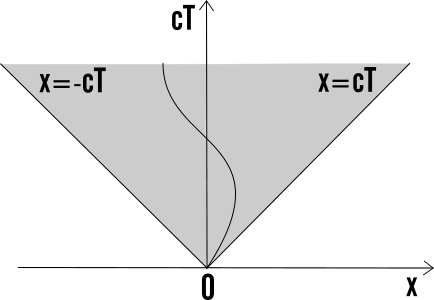
\includegraphics[width = .7\textwidth]{mink.png}
\end{figure}

\subsection{Il problema ``Vedere''}

La soluzione analitica al problema del “Vedere” non è complicata.
La condizione di visione si traduce nell’intersezione del moto del corpo in questione con il cono di luce passato

$$ | \vec{x}| = ct ,   t\leq 0 $$

Poichè il cono di luce è un invariante delle trasformazioni di Lorentz due osservatori nello stesso punto ma che
si muovono a velocità diverse “vedono” le stesse cose.
Inoltre poiché il tempo non puo’ assumere valori positivi il buffer della storia dell’oggetto puo’ essere unicamente
dedicato al suo passato rispetto al presente nel sistema privilegiato
Il problema quindi si traduce formalmente nella soluzione dell’equazione nel sistema di riferimento preferenziale

$$ | \vec{x(t)}| = ct $$

Per un corpo in moto rettilineo uniforme con legge oraria
$$  \vec{x(t)} = \vec{x_0} + \vec{v}(t-t_0)$$
$t$ risulta essere soluzione della seguente equazione di secondo grado
$$ (c^2-v^2)t^2-2(\vec{x_0} \cdot \vec{v}) t-x_0^2 =0 $$


\subsection{Il problema ``Presente''}
La soluzione al problema del presente risulta essere più complicata.
Le trasformazioni di Lorentz tridimensionali coinvolgono solo la coordinata temporale e l’asse spaziale parallelo
al moto dell’osservatore come nella formula di seguito
I calcoli per semplicità vengono eseguiti nel sistema di riferimento che è orientato con il versore $\hat{x}$ paralleoa al moto.

$$ 
\begin{matrix} 
x' = \gamma(x-\alpha t)\\
y' = y\\
z' = z\\
 t' = \gamma( t - \frac{\alpha}{c^2}x)\\
\end{matrix}
$$
la posizione di un generico corpo sarà quindi ora indicata come

$$ \vec{s(t)} =\left( \begin{matrix} x(t) \\ y(t) \\ z(t)\\ \end{matrix} \right)$$

Formalmente trovare la soluzione consiste nel risolvere per il presente l’equazione di Lorentz per la
trasformazione del tempo

$$ t' = \gamma( t - \frac{\alpha}{c^2}x(t)) $$

imponendo $t' =0$

$$ t=  \frac{\alpha}{c^2}x(t)  $$

dove $\alpha$ è la velocità dell’osservatore, e successivamente tranformare quell’evento per trovare ciò che verrà
visualizzato dall'osservatore in moto.
Per i corpi fissi la soluzione è di nuovo semplice e corrisponde alla nota “Contrazione delle lunghezze”
basterà eseguire una contrazione di $1/\gamma$ nella direzione del moto.

Per un oggetto in moto rettilineo uniforme con legge oraria
$$ x(t) = x_0 + v_x(t- t_0)$$

nella coordinata $x$, risolvendo per $t$ so ottiene

$$ t_p = \frac{\alpha}{c^2-\alpha v_x} (x_0-v_0 t_0) $$

L'oggetto viene quidni visto in

$$ \vec{s'} =\left( \begin{matrix} \gamma( x(t_p) - \alpha t_p) \\ y(t_p) \\ z(t_p)\\ \end{matrix} \right)$$

L’ultima difficoltà sorge dal fatto che un oggetto, seppur muovendosi più lento della luce, può nelle giuste
combinazioni di $\alpha$ e $v_x$ può essere visto dall’osservatore in movimento in un istante che per noi può essere
arbitrariamente lontano, sia nel passato che nel futuro.
Il buffer che tiene la storia dell’oggetto nel sistema di riferimento privilegiato sarà quindi interpretato e ripartito in
metà nel presente e metà nel passato

\section{Consigli di utilizzo}

Compilare da 0 il programma richiede un po’ di tempo, è quindi consigliabile lanciare make con l’opzione “-j”


Il programma fa’ largo uso dello heap attraverso puntatori condivisi, nel caso si trovasse a voler modificare
qualcosa, è possibile che il programma crashi all’avvio seppur compilando.
Nella maggior parte dei casi cio è risolvibile ricompilando tutti i file oggetto lanciando un comando “make
cleanall”

\end{document}